\documentclass[12pt]{article}
% Load packages
\usepackage{url}  % Formatting web addresses  
\usepackage{ifthen}  % Conditional 
\usepackage{multicol}   %Columns
\usepackage[utf8]{inputenc} %unicode support
\usepackage{amsmath}
\usepackage{amssymb}
\usepackage{epsfig}
\usepackage{epstopdf}
\usepackage{graphicx}
\usepackage[margin=0.1pt,font=footnotesize,labelfont=bf]{caption}
\usepackage{setspace}
%\usepackage{longtable}
\usepackage{colortbl}
%\usepackage{palatino,lettrine}
%\usepackage{times}
%\usepackage[applemac]{inputenc} %applemac support if unicode package fails
%\usepackage[latin1]{inputenc} %UNIX support if unicode package fails
\usepackage[wide]{sidecap}
%\usepackage[authoryear,round,comma,sort&compress]{natbib}
\usepackage[square,sort,comma,numbers]{natbib}
%\usepackage[authoryear,round]{natbib}
\usepackage{supertabular}
\usepackage{simplemargins}
\usepackage{comment}
\usepackage{lineno}

\urlstyle{rm}

%\textwidth = 6.50 in
%\textheight = 9.5 in
%\oddsidemargin =  0.0 in
%\evensidemargin = 0.0 in
%\topmargin = -0.50 in
%\headheight = 0.0 in
%\headsep = 0.25 in
%\parskip = 0.15in
%\linespread{1.75}
\doublespace

%\usepackage{geometry}
\usepackage{fullpage}

%\bibliographystyle{plain}
\bibliographystyle{plos2009}

\makeatletter
\renewcommand\subsection{\@startsection
	{subsection}{2}{0mm}
	{-0.05in}
	{-0.5\baselineskip}
	{\normalfont\normalsize\bfseries}}
\renewcommand\subsubsection{\@startsection
	{subsubsection}{2}{0mm}
	{-0.05in}
	{-0.5\baselineskip}
	{\normalfont\normalsize\itshape}}
\renewcommand\section{\@startsection
	{subsection}{2}{0mm}
	{-0.2in}
	{0.05\baselineskip}
	{\normalfont\large\bfseries}}	
\renewcommand\paragraph{\@startsection
	{paragraph}{2}{0mm}
	{-0.05in}
	{-0.5\baselineskip}
	{\normalfont\normalsize\itshape}}
\makeatother

%Review style settings
%\newenvironment{bmcformat}{\begin{raggedright}\baselineskip20pt\sloppy\setboolean{publ}{false}}{\end{raggedright}\baselineskip20pt\sloppy}

%Publication style settings

% Single space'd bib -
\setlength\bibsep{0pt}

\renewcommand{\rmdefault}{phv}\renewcommand{\sfdefault}{phv}
\newcommand{\norm}[1]{\left\lVert#1\right\rVert}

% Change the number format in the ref list -
\renewcommand{\bibnumfmt}[1]{#1.}

% Change Figure to Fig.
\renewcommand{\figurename}{Fig.}

% Begin ...
\begin{document}
\begin{titlepage}
{\par\centering\textbf{\Large Dynamic Modeling of Biochemical Networks using Effective Kinetic Models}}
\vspace{0.05in}
{\par \centering \large{Joseph A. Wayman, Adithya Sagar and Jeffrey D. Varner$^{*}$}}
\vspace{0.10in}
{\par \centering \large{School of Chemical and Biomolecular Engineering}}
{\par \centering \large{Cornell University, Ithaca NY 14853}}
\vspace{0.1in}
{\par \centering \textbf{Running Title:}~Effective models of metabolism}
\vspace{0.1in}
{\par \centering \textbf{To be submitted:}~\emph{Processes}}
\vspace{0.5in}
{\par \centering $^{*}$Corresponding author:}
{\par \centering Jeffrey D. Varner,}
{\par \centering Associate Professor, School of Chemical and Biomolecular Engineering,}
{\par \centering 244 Olin Hall, Cornell University, Ithaca NY, 14853} 
{\par \centering Email: jdv27@cornell.edu} 
{\par \centering Phone: (607) 255 - 4258}
{\par \centering Fax: (607) 255 - 9166}
\end{titlepage}
\date{}
\thispagestyle{empty}
\pagebreak
%%%%%%%%%%%%%%%%%%%%%%%%%%%%%%%%%%%%%%%%%%%%%%%%%%%%%%%%%%%%%%%%%%%%%%%%%%%%%%%%%%%%%%%%%%%%%%%%%%%%%%%%%%%
%%%%%%%%%%%%%%%%%%%%%%%%%%%%%%%%%%%%%%%%%%%%%%%%%%%%%%%%%%%%%%%%%%%%%%%%%%%%%%%%%%%%%%%%%%%%%%%%%%%%%%%%%%%
\section*{Abstract}

{\noindent \textbf{Keywords:}~Cell free metabolism, Mathematical modeling}

\pagebreak

\setcounter{page}{1}

\linenumbers

\section*{Introduction}
Biochemical processes are widely used in biotechnology to produce an array of products including commodity chemicals and protein therapeutics.
However, whole-cell processes share the central limitation of requiring cell growth, 
which redirects resources away from product synthesis, and cell walls, which complicate interrogation and control of intracellular metabolic processes.
On the other hand, cell-free metabolic systems offer many advantages over traditional in vivo production methods. 
For example, cell-free systems can direct scarce metabolic resources exclusively towards a single product of interest. 
Moreover, with no cell wall, cell free systems can more easily be interrogated, and substrates of the metabolite processes directly controlled.
Cell free production offers the unique opportunity to study metabolism without the complication of cell growth and gene expression processes.
For modeling, this implies that we need only consider allosteric regulation of enzyme activity when building and testing cell free metabolic models.
Of course, modeling allosteric mechanisms is itself a difficult problem when the model is at a whole genome scale. To address this problem, we have developed a
an approach based upon the constrained fuzzy logic framework of Morris and Lauffenburger [REFHERE].

In this study, we present an effective biochemical network modeling framework that integrates classical kinetic modeling with rules based approaches.
[FINISH ME]

\clearpage

\section*{Results}

\subsection*{Formulation and properties of cell free effective models.}
We developed two proof-of-concept metabolic networks to investigate the features of our effective biochemical network modeling approach (Fig. \ref{fig-networks}).
In both examples, substrate $S$ was converted to the end-products $P_{1}$ and $P_{2}$ through a series of enzymatically catalyzed reactions, 
including a branch point at hypothetical metabolite $M_{2}$. 
Several of these reactions involved cofactor dependence ($AH$ or $A$), and various allosteric regulation mechanisms. 
Network A included feedback inhibition of the initial pathway enzyme ($E_{1}$) by pathway end products $P_{1}$ and $P_{2}$ (Fig. \ref{fig-networks}A).
On the other hand, network B involved feedback inhibition of $E_{1}$ by $P_{2}$ and $E_{6}$ by $P_{1}$ (Fig. \ref{fig-networks}B). 
In both networks, branch point enzymes $E_{3}$ and $E_{6}$ were subject to feed-forward activation by cofactor $AH$.
Lastly, enzyme activity was assumed to decay according to a first-order rate law in both cases. 
Allosteric regulation of enzyme activity was represented using a novel rule-based strategy, similar in spirit to the 
Constrained Fuzzy Logic (cFL) approach of Lauffenberger and coworkers \citep{Morris:2011aa}. 
In this formulation, Hill-like transfer functions were used to calculate the influence of metabolite abundance upon target enzyme activity. 
When an enzyme was potentially sensitive to more than one regulatory influence, logical rules were used to select which transfer function regulated enzyme 
activity at any given time (Fig. \ref{fig-control-schematic}).      
Thus, our test networks involved important features such as cofactor recycling, enzyme activity and metabolite dynamics, 
as well as multiple overlapping allosteric regulatory mechanisms.  
As such, developing our effective modeling approach using these simple problems gave us valuable insight into the development of larger network models, 
without the complication of network size. 

The rule based regulatory strategy approximated the behavior of classical allosteric activation and inhibition mechanisms (Fig. \ref{fig-kinetics-simulations}).  
We first explored feed-forward substrate activation of enzyme activity (for both positive and negative cooperativity). 
Consistent with classical data, the rule based strategy predicted a sigmoidal relationship between substrate abundance 
and reaction rate as a function of the cooperativity parameter (Fig. \ref{fig-kinetics-simulations}A). 
For cooperativity parameters less than unity, increased substrate abundance \textit{decreased} the reaction rate. This was consistent with the idea that
substrate binding \textit{decreases} at regulatory sites negatively impacts the ability of the enzyme to bind substrate at the active site. 
On the other hand, as the cooperativity parameter increased past unity, the rate of conversion of substrate $S$ to product $P$ by enzyme $E$ approached a step function.
In the presence of an inhibitor, the rule based strategy predicted non-competitive like behavior as a function of the 
cooperativity parameter (Fig. \ref{fig-kinetics-simulations}B). 
When the control gain parameter, $\kappa_{ij}$ in Eqn. \eqref{eqn:control-factor}, was greater than unity, the inhibitory force was
directly proportional to the cooperativity parameter, $\eta$ in Eqn. \eqref{eqn:control-factor}. 
Thus, as the cooperativity parameter increased, the maximum reaction rate decreased (Fig. \ref{fig-kinetics-simulations}B, orange).
However, when the gain parameter was less than unity, enzyme inhibition increased with \textit{decreasing} cooperativity, 
i.e., smaller $\eta$ yielded increased inhibition (Fig. \ref{fig-kinetics-simulations}B).
Interestingly, our rule based approach was unable to directly simulate competitive inhibition of enzyme activity. 
For competitive inhibitors, the kinetic component of our rate, $\bar{r}_{j}$ in \eqref{eqn:rate-factor}, could be modified to account 
for the inhibition (data not shown). 
Taken together, the rule based strategy captured classical regulatory patterns for both enzyme activation and inhibition. 
Thus, we are able to model complex kinetic phenomena such as ultrasensitivity, despite an effective description of reaction kinetics. 
    
End product yield was controlled by feedback inhibition, while selectivity was controlled by branch point enzyme inhibition (Fig. \ref{fig-onoff-simulations}).
A critical test of our modeling approach was to simulate networks with known behavior. If we cannot reproduce the expected behavior of simple networks, then our
effect modeling strategy, and particularly the rule-based approximation of allosteric regulation, will not be feasible for large scale problems.
We considered two cases,  control on/off, for each network configuration. 
Each of these cases had identical kinetic parameters and initial conditions; 
the \textit{only} differences between the cases was the allosteric regulation rules, and the control parameters associated with these rules. 
As expected, end product accumulation was larger for network A when the control was off (no feedback inhibition of $E_{1}$ by $P_{1}$ and $P_{2}$),
as compared to the on case (Fig. \ref{fig-onoff-simulations}A). We found this behavior was robust to the choice of underlying kinetic parameters, 
as we observed that same qualitative response across an ensemble of randomized parameter sets (N = 100). 
The control on/off response of network B was more subtle. In the off case, the behavior was qualitatively similar to network A. 
However, for the on case, flux was diverted away from $P_{2}$ formation by feedback inhibition of $E_{6}$ activity at the $M_{2}$ branch point by $P_{1}$ (Fig. \ref{fig-onoff-simulations}B).
Lower $E_{6}$ activity at the $M_{2}$ branch point allowed more flux toward $P_{1}$ formation, hence the yield of $P_{1}$ also increased (Fig. \ref{fig-onoff-simulations}C).
Again, the control on/off behavior was robust to the values of the kinetic parameters, as the same qualitative trend was conserved across 
an ensemble of possible randomized kinetic parameters (N = 100). Taken together, these simulations suggested that the rule based allosteric control 
concept could robustly capture expected feedback behavior.


\subsection*{Estimating parameters and effective allosteric regulatory structures.}
A critical challenge for any dynamic model is the estimation of kinetic parameters. 
For metabolic processes, there is also the added challenge of identifying the regulation and control structures that manage metabolism.  
Of course, these issues are not independent; any description of enzyme activity regulation will be a function of system state, which
in turn depends upon the kinetic parameters. For cell free systems, regulated gene expression has been removed, however, enzyme activity regulation is still operational. 
We explored this linkage by estimating model parameters from synthetic data using both network
structures. We generated noise-corrupted synthetic measurements of the substrate $S$, intermediate $M_{5}$ and end-product $P_1$ approximately every 20 min using
network A. We then generated an ensemble of model parameter estimates by minimizing the difference between model simulations and the synthetic data using particle swarm
optimization, starting from random initial guesses. The estimation of kinetic parameters was sensitive to the choice of regulatory structure (Fig. \ref{fig-parameter-fit}).
PSO identified an ensemble of parameters that bracketed the mean of the synthetic measurements in less than 1000 iterations when the control structure was correct (Fig. \ref{fig-parameter-fit}A and B).However, when there was network mismatch (network B fit against network A synthetic data), PSO unable to identify an ensemble, all else being the same (Fig. \ref{fig-parameter-fit}C and D). Interestingly, the particle swarm generated a \textit{sloppy} parameter ensemble, in the absence of network mismatch (Fig. ZZZ). 
Taken together, ... [FINISH].

We modified our particle swarm identification strategy to simultaneously search over both kinetic parameters and putative control structures.
In addition to our initial networks, we constructed three additional presumptive network models, each with the same enzymatic connectivity but different allosteric 
regulation of the pathway enzymes (Fig. \ref{fig-alternative-networks}). 
We then initialized a population of particles, each with one of the five potential regulatory programs, and randomized kinetic parameters.
Thus, we generated an initial population of particles that had \textit{both} different kinetic parameters as well as different control structures. 
We biased the distribution of the particle population according to our \textit{a~prior} belief of the correct regulatory program.
To this end, we considered three different priors, a uniform distribution where each putative regulatory structure represented 20\% of the population, and
two mixed distributions that were either positively or negatively biased towards the correct structure (network A).
In both the positively biased, and uniform cases the particle swarm clearly differentiated between the true or closely related structures and those that were materially different (Fig. \ref{fig-control-search}).  As expected, the positively biased population (40\% of the initial particle population seeded with network A) gave the best results, where the correct structure was preferentially identified (Fig. \ref{fig-control-search}A). 
On the other hand, when given a uniform distribution, 
the PSO approach identified a combination of network A (ZZ) and network C (YY) as the most likely control structures (Fig. \ref{fig-control-search}B).
Network A and C differ by the regulatory connection between the end-product $P_2$ and enzyme $E_{1}$; in network A $P_{2}$ was assumed to inhibit $E_{1}$ while in network C $P_{2}$ was assumed to activate $E_{1}$.  Lastly, when the initial population was biased towards a completely incorrect structure (initial population seeded with 40\% network B), 
the particle swarm \textit{misidentified} the correct allosteric structure (Fig. \ref{fig-control-search}C). 




\clearpage

\section*{Discussion}
In this study, we proposed a effective modeling strategy to dynamically simulate cell free metabolic networks. 
We tested this strategy using two proof of concept metabolic networks.
In both networks, substrate $S$ was converted to the end-products $P_{1}$ and $P_{2}$ through a series of enzymatically catalyzed reactions, 
including a branch point at hypothetical metabolite $M_{2}$. While both networks had the same enzymatic connectivity, that had differing control structures.
[FINISH]

Cybernetic models, other dynamic models of metabolism. 

While the results of this study were encouraging, there are several critical next steps that must be accomplished before we can model genome scale cell free metabolic networks.
[FINISH]

\clearpage

\section*{Materials and Methods}

\subsection*{Formulation and solution of the model equations.}
We used ordinary differential equations (ODEs) to model the time evolution of metabolite ($x_{i}$) and scaled enzyme abundance ($\epsilon_{i}$) in hypothetical cell free
metabolic networks:
\begin{eqnarray}
	\frac{dx_{i}}{dt} & = & \sum_{j = 1}^{\mathcal{R}}\sigma_{ij}r_{j}\left(\mathbf{x},\mathbf{\epsilon},\mathbf{k}\right)\qquad{i=1,2,\hdots,\mathcal{M}}\\
	\frac{d\epsilon_{i}}{dt} & = & -\lambda_{i}\epsilon_{i}\qquad{i = 1,2,\hdots,\mathcal{E}}
\end{eqnarray}where $\mathcal{R}$ denotes the number of reactions, $\mathcal{M}$ denotes the number of metabolites and $\mathcal{E}$ denotes the number of
enzymes in the model. The quantity $r_{j}\left(\mathbf{x},\mathbf{\epsilon},\mathbf{k}\right)$ 
denotes the rate of reaction $j$. Typically, reaction $j$ is a non-linear function of metabolite and enzyme abundance, as well as unknown kinetic parameters 
$\mathbf{k}$ ($\mathcal{K}\times{1}$).
The quantity $\sigma_{ij}$ denotes the stoichiometric coefficient for species $i$ in reaction $j$. If 
$\sigma_{ij}>0$, metabolite $i$ is produced by reaction $j$. Conversely, if $\sigma_{ij}>0$, metabolite $i$ is consumed by reaction $j$, while $\sigma_{ij} = 0$ indicates
metabolite $i$ is not connected with reaction $j$. Lastly, $\lambda_{i}$ denotes the scaled enzyme degradation constant. The system material balances were subject to the
initial conditions $\mathbf{x}\left(t_{o}\right) = \mathbf{x}_{o}$ and $\mathbf{\epsilon}\left(t_{o}\right) = \mathbf{1}$ (initially we have 100\% cell-free enzyme abundance).

Each reaction rate was written as the product of two terms, a kinetic term ($\bar{r}_{j}$) and a regulatory term ($v_{j}$):
\begin{equation}\label{eqn:rate-factor}
	r_{j}\left(\mathbf{x},\mathbf{\epsilon},\mathbf{k}\right) = \bar{r}_{j}v_{j}
\end{equation}We used multiple saturation kinetics to model the reaction term $\bar{r}_{j}$:
\begin{equation}\label{eqn:rate-bar}
	\bar{r}_{j} = k_{j}^{max}\epsilon_{i}\left(\prod_{s\in{m_{j}^{-}}}\frac{x_{s}}{K_{js} + x_{s}}\right)
\end{equation}where $k_{j}^{max}$ denotes the maximum rate for reaction $j$, $\epsilon_{i}$ denotes the scaled enzyme activity which catalyzes reaction $j$, and
$K_{js}$ denotes the saturation constant for species $s$ in reaction $j$. 
The product in Eqn. \eqref{eqn:rate-bar} was carried out over the set of \textit{reactants} for reaction $j$ (denoted as $m_{j}^{-}$). 

The allosteric regulation term $v_{j}$ depended upon the combination of factors which influenced the activity of enzyme $i$.
For each enzyme, we used a rule based approach to select from competing control factors (Fig. \ref{fig-control-schematic}). 
If an enzyme was activated by $m$ metabolites, we modeled this activation as:
\begin{equation}
	v_{j} = \max\left(f_{1j}\left(x\right),\hdots,f_{mj}\left(x\right)\right)
\end{equation}where $0\leq f_{ij}\left(x\right)\leq 1$ was a regulatory transfer function that calculated the influence of metabolite $i$ on the activity of enzyme $j$. 
Conversely, if enzyme activity was inhibited by a $m$ metabolites, we modeling this inhibition as:
\begin{equation}
	v_{j} = 1 - \max\left(f_{1j}\left(x\right),\hdots,f_{mj}\left(x\right)\right)
\end{equation}Lastly, if an enzyme had both $m$ activating and $n$ inhibitory factors, we modeled the regulatory term as:
\begin{equation}
	v_{j} = \min\left(u_{j},d_{j}\right)
\end{equation}where:
\begin{eqnarray}
	u_{j} &=& \max_{j^{+}}\left(f_{1j}\left(x\right),\hdots,f_{mj}\left(x\right)\right) \\
	d_{j} &=& 1 - \max_{j^{-}}\left(f_{1j}\left(x\right),\hdots,f_{nj}\left(x\right)\right)
\end{eqnarray}The quantities $j^{+}$ and $j^{-}$ denoted the sets of activating, and inhibitory factors for enzyme $j$. 
If an enzyme had no allosteric factors, we set $v_{j} = 1$.
There are many possible functional forms for $0\leq f_{ij}\left(x\right)\leq 1$. 
However, in this study, each individual transfer function took the form:
\begin{equation}\label{eqn:control-factor}
	f_{i}\left(\mathbf{x}\right) = \frac{\kappa_{ij}^{\eta}x_{j}^{\eta}}{1 + \kappa_{ij}^{\eta}x_{j}^{\eta}}
\end{equation}where $x_{j}$ denotes the abundance of metabolite $j$, and $\kappa_{ij}$ and $\eta$ are control parameters. 
The $\kappa_{ij}$ parameter was species gain parameter, while $\eta$ was a cooperativity parameter (similar to a Hill coefficient).
The model equations were encoded using the Octave programming language, and solved using the LSODE routine in Octave \citep{Octave:2014}.

\subsection*{Estimation of model parameters and structures from synthetic experimental data.}
Model parameters were estimated by minimizing the difference between simulations and synthetic experimental data (squared residual):
\begin{equation}\label{eqn:objective-function}
	\min_{\mathbf{k}} \sum_{\tau=1}^{\mathcal{T}}\sum_{j=1}^{\mathcal{S}}\left(\frac{\hat{x}_{j}\left(\tau\right) - x_{j}\left(\tau,\mathbf{k}\right)}{\omega_{j}\left(\tau\right)}\right)^{2}
\end{equation}where $\hat{x}_{j}\left(\tau\right)$ denotes the measured value of species $j$ at time $\tau$, $x_{j}\left(\tau,\mathbf{k}\right)$ denotes the simulated 
value for species $j$ at time $\tau$, and $\omega_{j}\left(\tau\right)$ denotes the experimental measurement variance for species $j$ at time $\tau$. The outer summation is respect to
time, while the inner summation is with respect to state. We approximated a realistic model identification scenario, assuming noisy experimental data, 
limited sampling resolution (approximately 20 minutes per sample) and a limited number of measurable metabolites. 

We minimized the model residual using Particle swarm optimization (PSO) \citep{PSO}.
PSO uses a \textit{swarming} metaheuristic to explore parameter spaces. 
A strength of PSO is its ability to find the global minimum, even in the presence of potentially many local minima, by communicating the local
error landscape experienced by each particle collectively to the swarm. Thus, PSO acts both as a local and a global search algorithm. 
For each iteration, particles in the swarm compute their local error by evaluating the model equations using their specific parameter vector realization.
From each of these local points, a globally best error is identified. Both the local and global error 
are then used to update the parameter estimates of each particle using the rules:
\begin{eqnarray}
	\mathbf{\Delta}_{i} &=&\theta_{1}\mathbf{\Delta}_{i} + \theta_{2}\mathbf{r}_{1}\left(\mathcal{L}_{i} - \mathbf{k}_{i}\right) + \theta_{3}\mathbf{r}_{2}\left(\mathcal{G} - \mathbf{k}_{i}\right) \\
	\mathbf{k}_{i} &=& \mathbf{k}_{i} + \mathbf{\Delta}_{i}
\end{eqnarray}where $\left(\theta_{1},\theta_{2},\theta_{3}\right)$ are adjustable parameters, $\mathcal{L}_{i}$ denotes local best solution found by particle $i$, and
$\mathcal{G}$ denotes the best solution found over the entire population of particles. The quantities $r_{1}$ and $r_{2}$ denote uniform random vectors with the same dimension as the number of unknown model
parameters ($\mathcal{K}\times{1}$). In thus study, we used $\left(\theta_{1},\theta_{2},\theta_{3}\right) = \left(1.0, 0.05564, 0.02886\right)$, which was taken from XXX. The quality of parameter
estimates was measured using two criteria, goodness of fit (model residual) and angle between the estimated parameter vector $\mathbf{k}_{j}$ and the true parameter set $\mathbf{k}^{*}$:
\begin{equation}
	\alpha_{j} = cos^{-1}\left(\frac{\mathbf{k}_{j}\cdot{\mathbf{k^{*}}}}{\norm{\mathbf{k}_{j}}\norm{\mathbf{k^{*}}}}\right)
\end{equation}If the candidate parameter set $\mathbf{k}_{j}$ were perfect, the residual between the model and synthetic data 
and the angle between $\mathbf{k}_{j}$ and the true parameter set $\mathbf{k}^{*}$ would be equal to zero.

We modified our PSO implementation to simultaneously search over kinetic parameters and putative model control structures.
In the combined case, each particle potentially carried a different model realization in addition to a different kinetic parameter vector. 
We kept the update rules the same (along with the update parameters). 
Thus, each particle competed on the basis of goodness of fit, which allowed different model structures to contribute to the overall behavior of the swarm. 
We considered five possible model structures (A through E), where network A was the correct formulation (used to generate the synthetic data). 
We considered a population N = 100 particles, where each particle in the swarm was assigned a model structure, and a random parameter vector.
The PSO algorithm, model equations, and the objective function were encoded and solved in the Octave programming language \citep{Octave:2014}.

\section*{Acknowledgements}
This study was supported by the National Science Foundation GK12 award (DGE-1045513) 
and by the National Science Foundation CAREER award (FILLMEIN).

\clearpage
%\bibliographystyle{plain}
%\bibliographystyle{IEEEbib}

\bibliography{References_v1}

%\begin{comment}

\clearpage

\begin{figure}
\centering
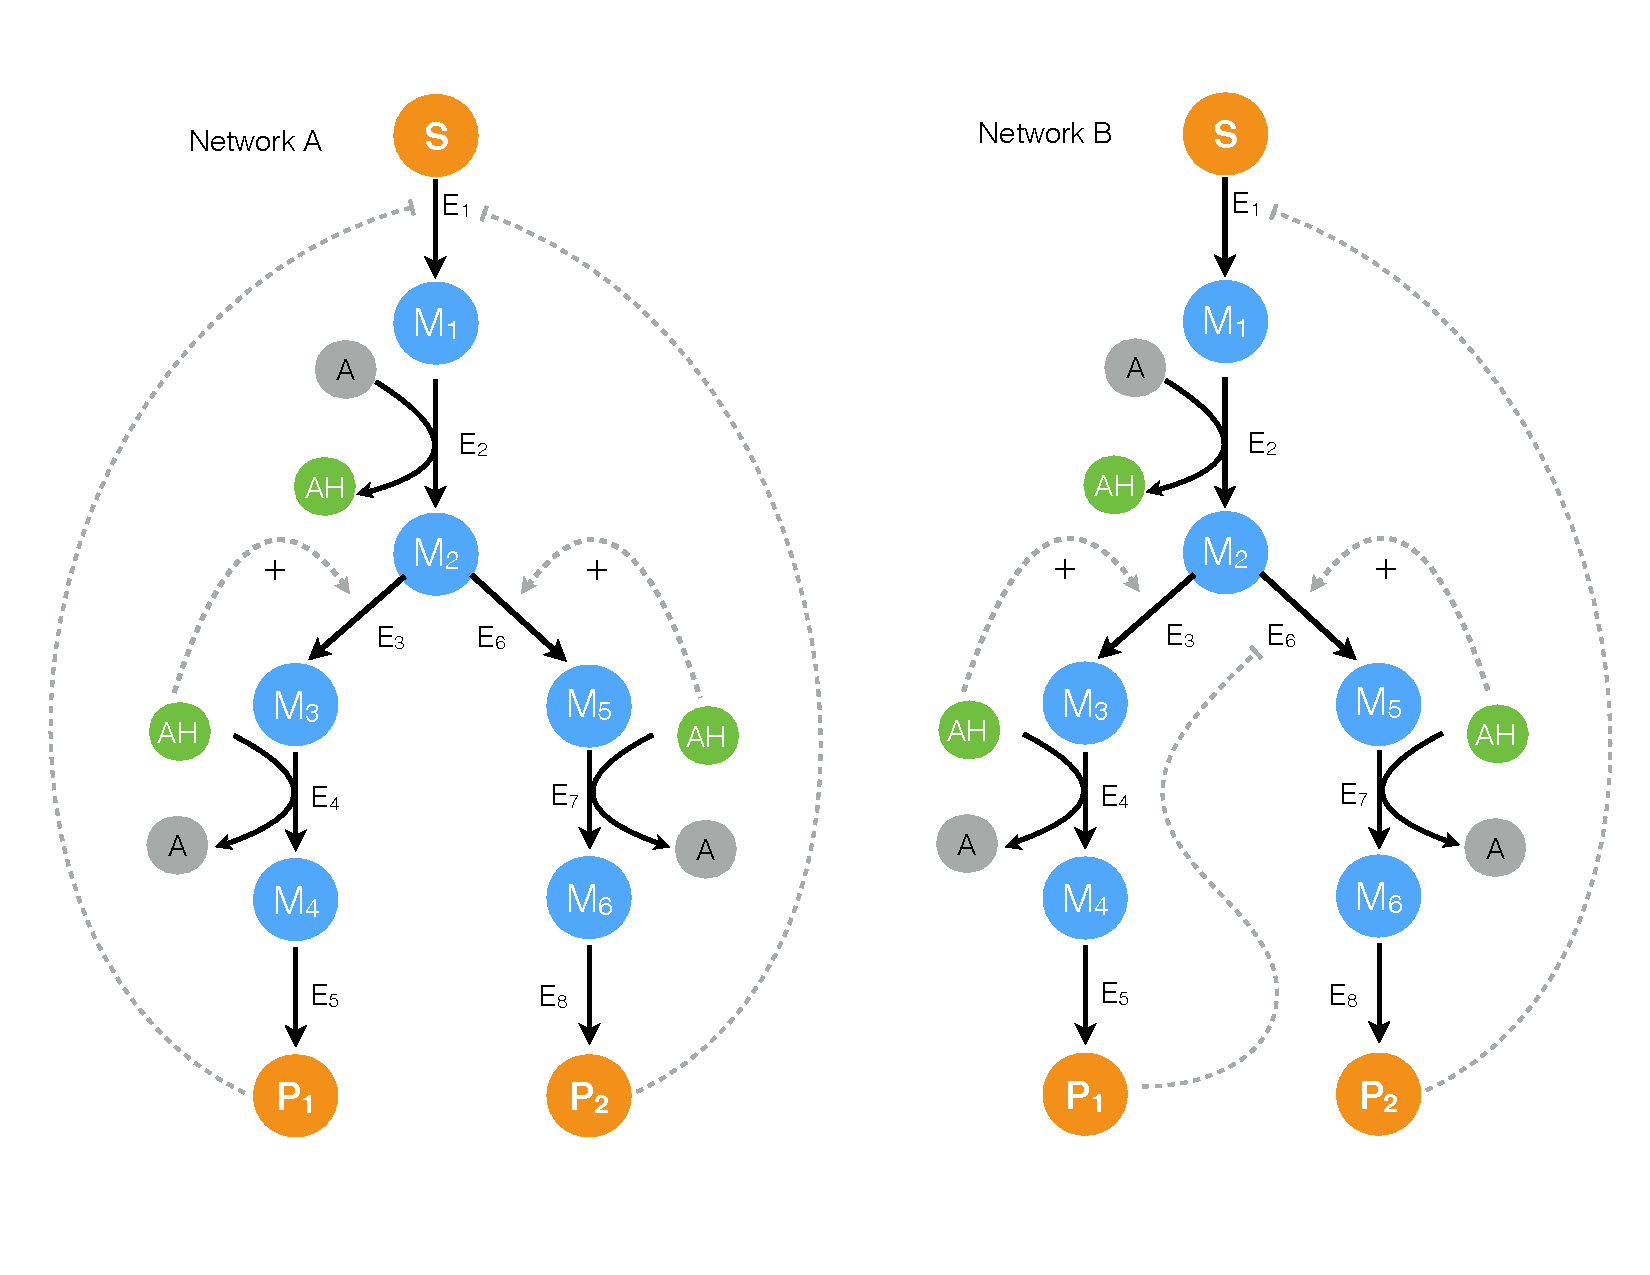
\includegraphics[width=1.0\textwidth]{./figs/Figure-1-Networks.pdf}
\caption{Proof of concept cell-free metabolic networks considered in this study. Substrate $S$ is converted to products $P_{1}$ and $P_{2}$ through a series of chemical conversions
catalyzed by enzyme(s) $E_{j}$. The activity of the pathway enzymes is subject to both positive and negative allosteric regulation. }\label{fig-networks}
\end{figure}

\clearpage

\begin{figure}
\centering
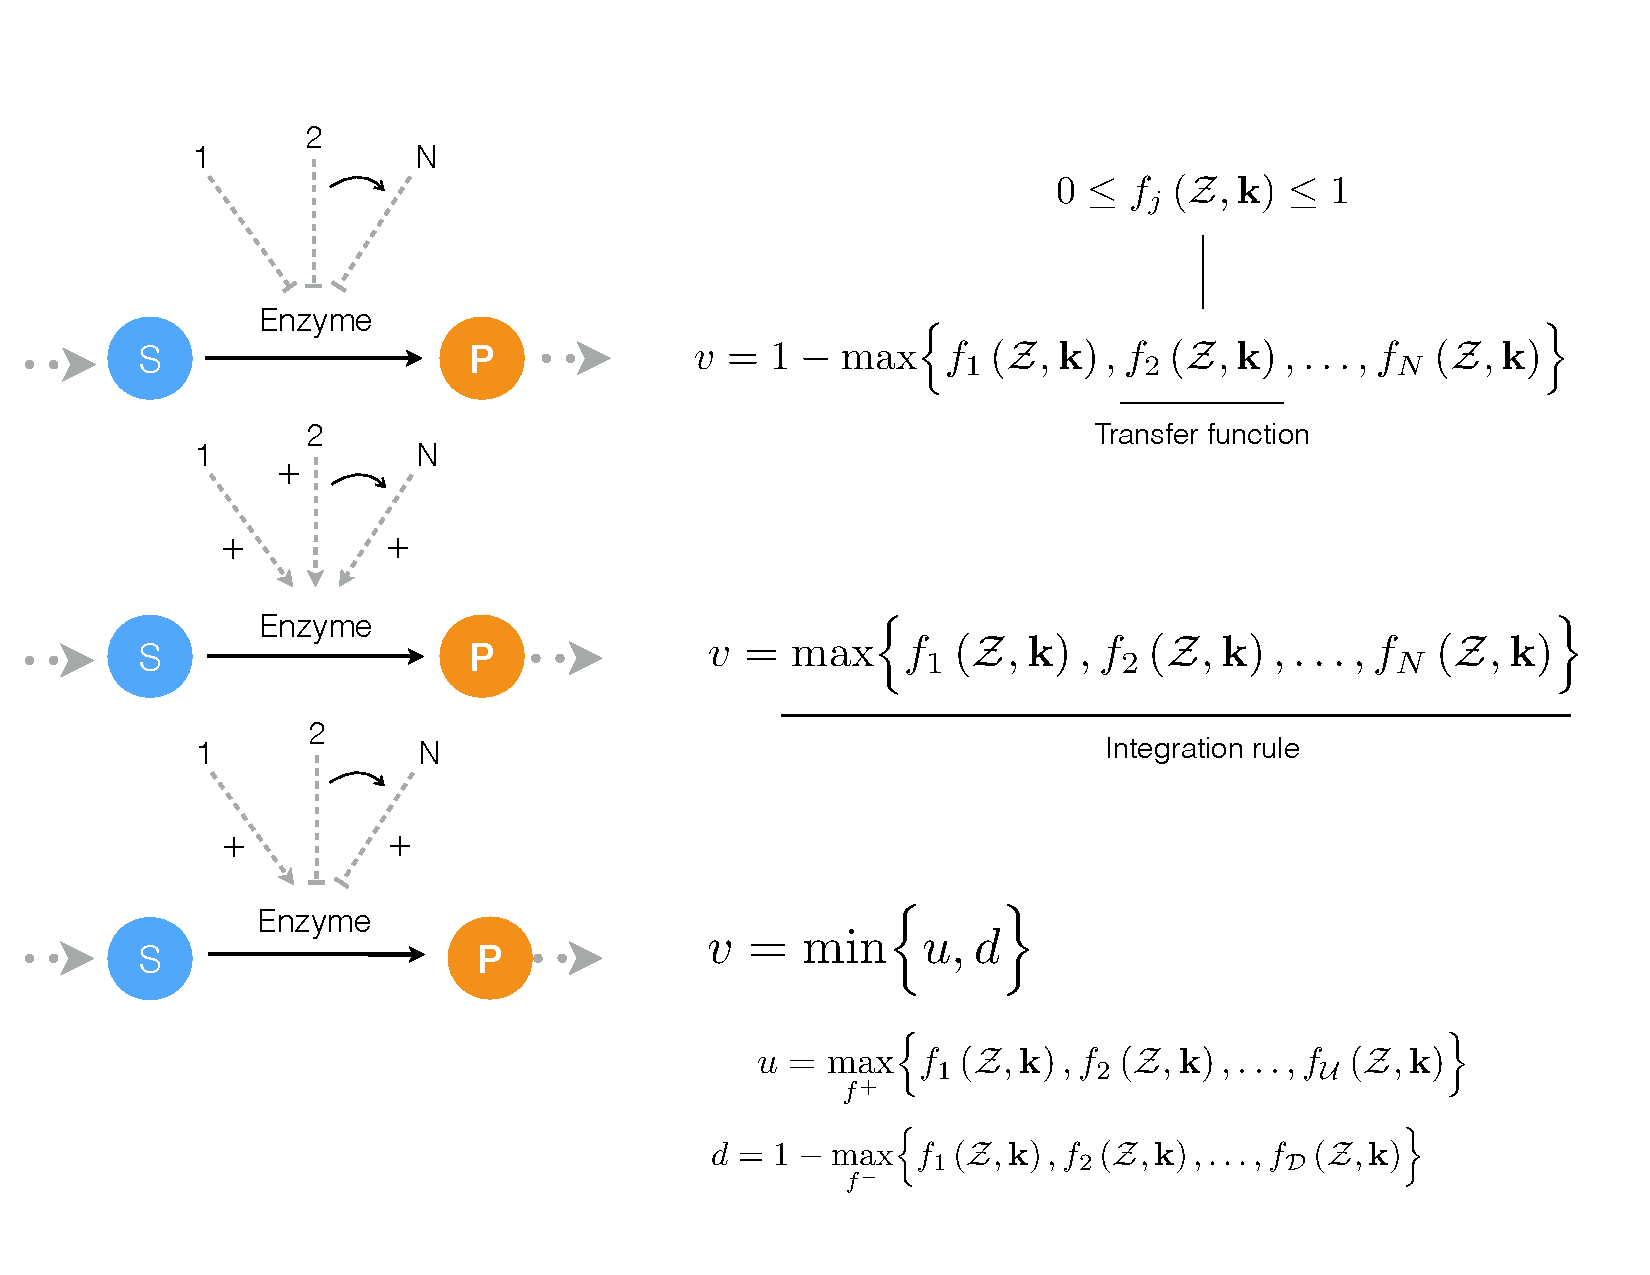
\includegraphics[width=1.0\textwidth]{./figs/Figure-2-ControlSchematic.pdf}
\caption{Schematic of rule based allosteric enzyme activity control laws. 
Traditional enzyme kinetic expressions e.g., Michaelis–Menten or multiple saturation kinetics are multiplied by an enzyme activity control variable $0 \leq v_{j} \leq 1 $. 
Control variables are functions of many possible regulatory factors encoded by arbitrary functions of the form $0\leq f_{j}\left(\mathcal{Z}\right)\leq 1$.
At each simulation time step, the $v_{j}$ variables are calculated by evaluating integration rules such as the max or min of the set of factors $f_{1},\hdots$ 
influencing the activity of enzyme $E_{j}$. }\label{fig-control-schematic}
\end{figure}

\clearpage

\begin{figure}
\centering
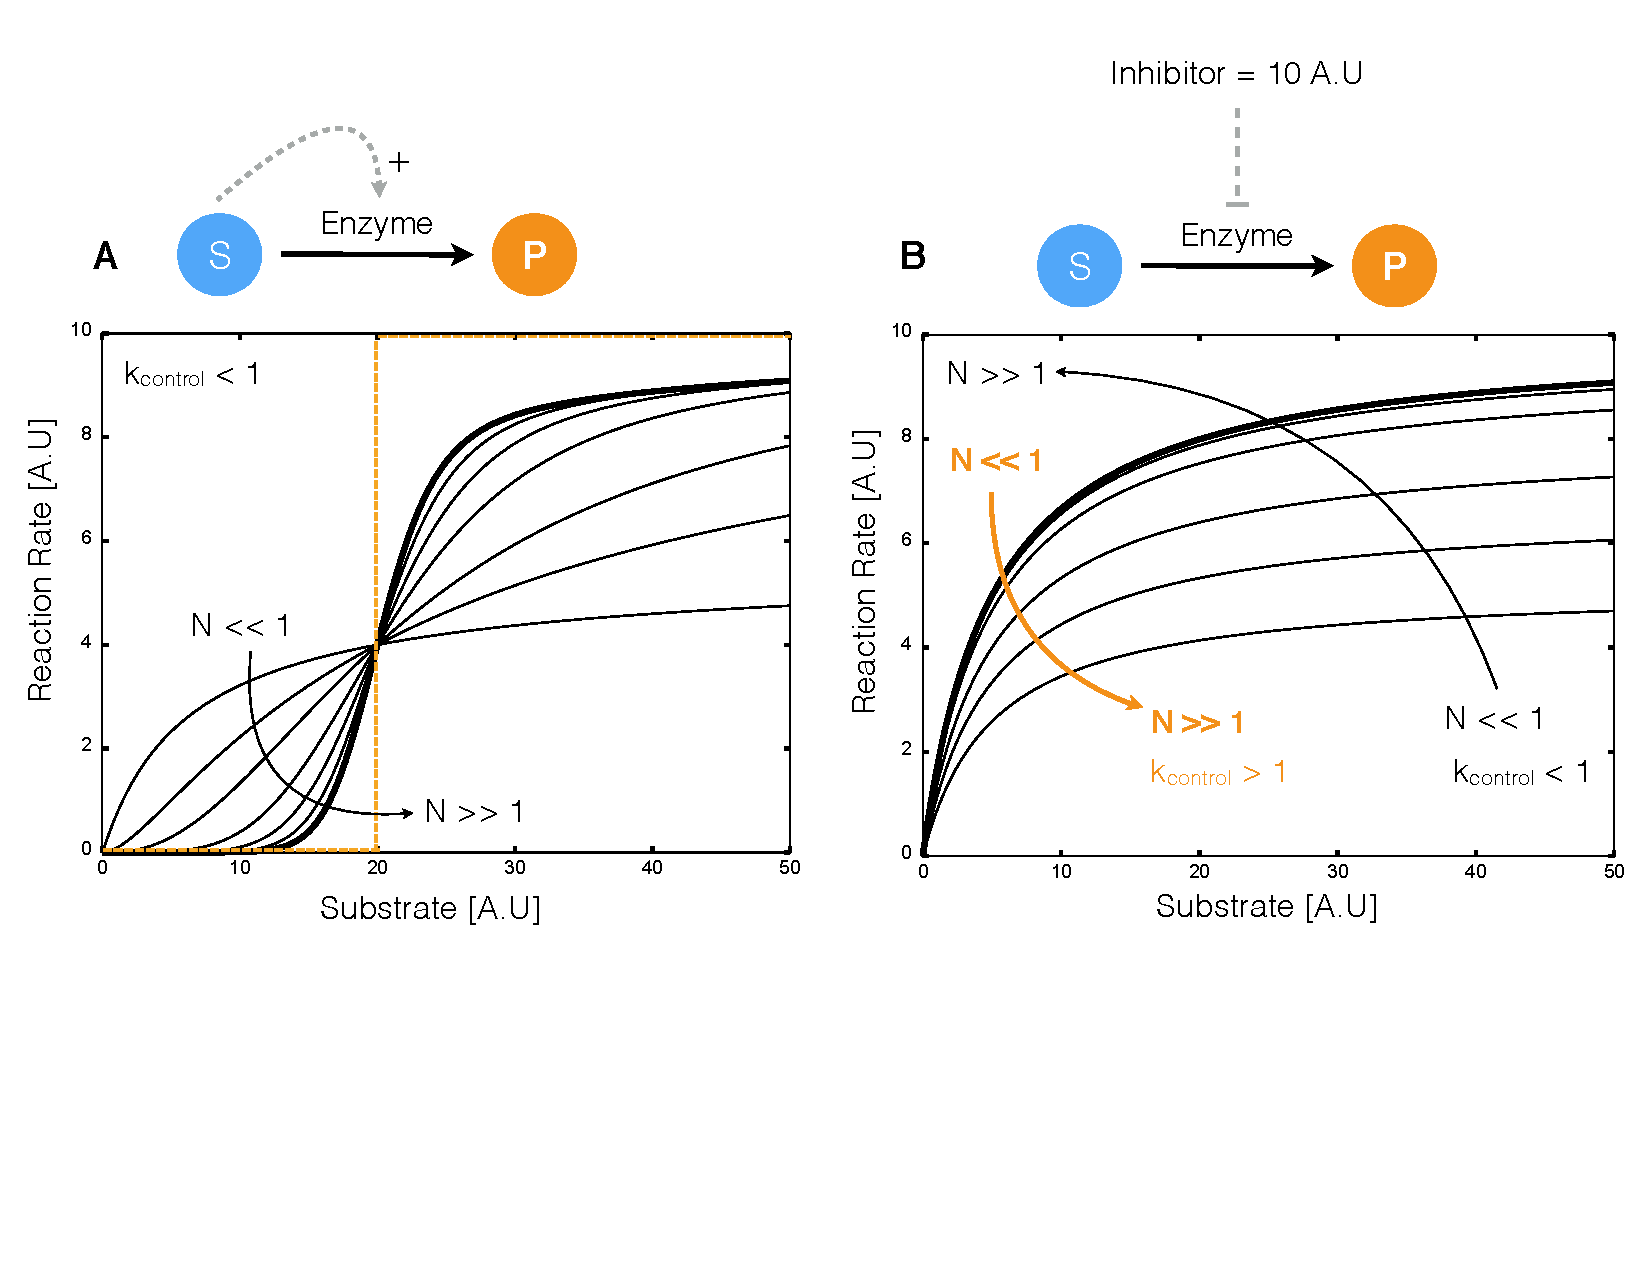
\includegraphics[width=1.0\textwidth]{./figs/Figure-3-EnzymeKinetics.pdf}
\caption{Kinetics of simple transformations in the presence of activation and inhibition. 
\textbf{A}:The conversion of substrate $S$ to product $P$ by enzyme $E$ was activated by $S$. 
For a fixed control gain parameter $k_{control}$, the reaction rate approached a step for increasing control order $N$. 
\textbf{B}:The conversion of substrate $S$ to product $P$ by enzyme $E$ with inhibitor $I$. 
For a fixed control gain parameter $k_{control}$, the reaction rate approximated non-competitive inhibition for increasing control order $N$. 
}\label{fig-kinetics-simulations}
\end{figure}

\clearpage

\begin{figure}
\centering
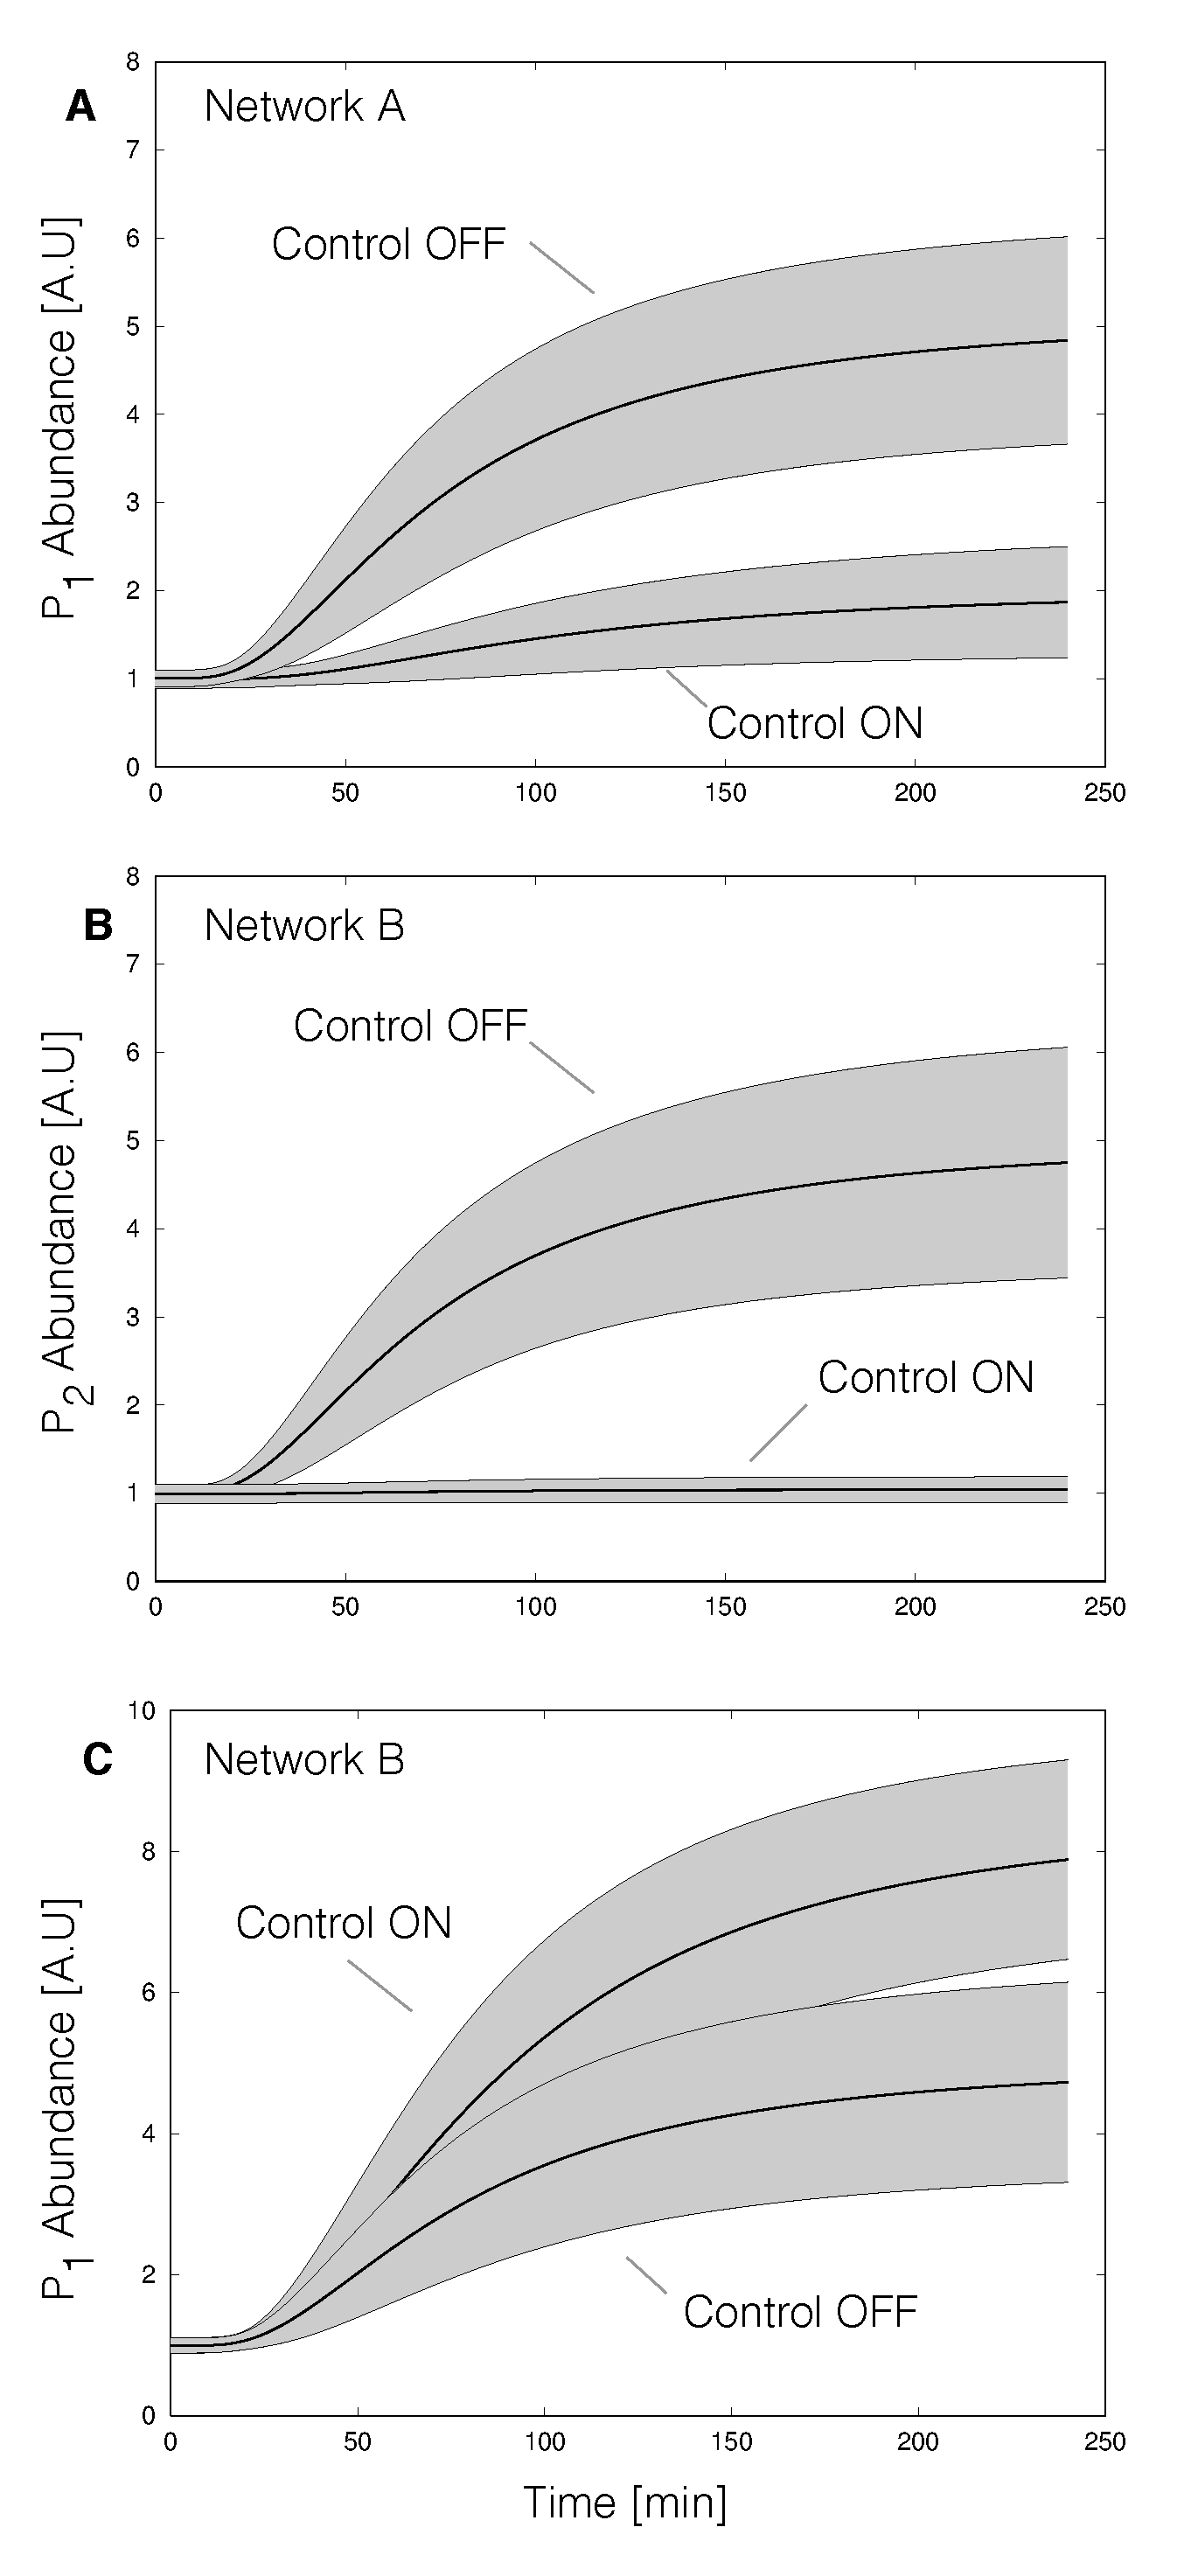
\includegraphics[width=0.50\textwidth]{./figs/Figure-4-OnOffSimulations.pdf}
\caption{ON/OFF control simulations for network A and network B for an ensemble of kinetic parameter sets versus time (N = 100). 
For each case, N = 100 simulations were conducted using kinetic and initial conditions generated randomly from a hypothetical true parameter set. 
The gray area represents $\pm$ one standard deviation surrounding the mean. 
Control parameters were fixed during the ensemble calculations.
\textbf{A}: End-product P$_{1}$ abundance versus time for Network A. 
The abundance of P$_{1}$ decreased with end-product inhibition of $E_{1}$ activity (Control-ON) versus the no inhibition case (Control-OFF). 
\textbf{B}: End-product P$_{2}$ abundance versus time for Network B. Inhibition of branch point $E_{6}$ by end-product P$_{1}$ decreased P$_{2}$ abundance (Control-ON) versus the
no inhibition case (Control-OFF).
\textbf{C}: End-product P$_{1}$ abundance versus time for Network A. 
Inhibition of branch point $E_{6}$ by end-product P$_{1}$ decreased P$_{1}$ abundance (Control-ON) versus the no inhibition case (Control-OFF).
}\label{fig-onoff-simulations}
\end{figure}

\clearpage

\begin{figure}
\centering
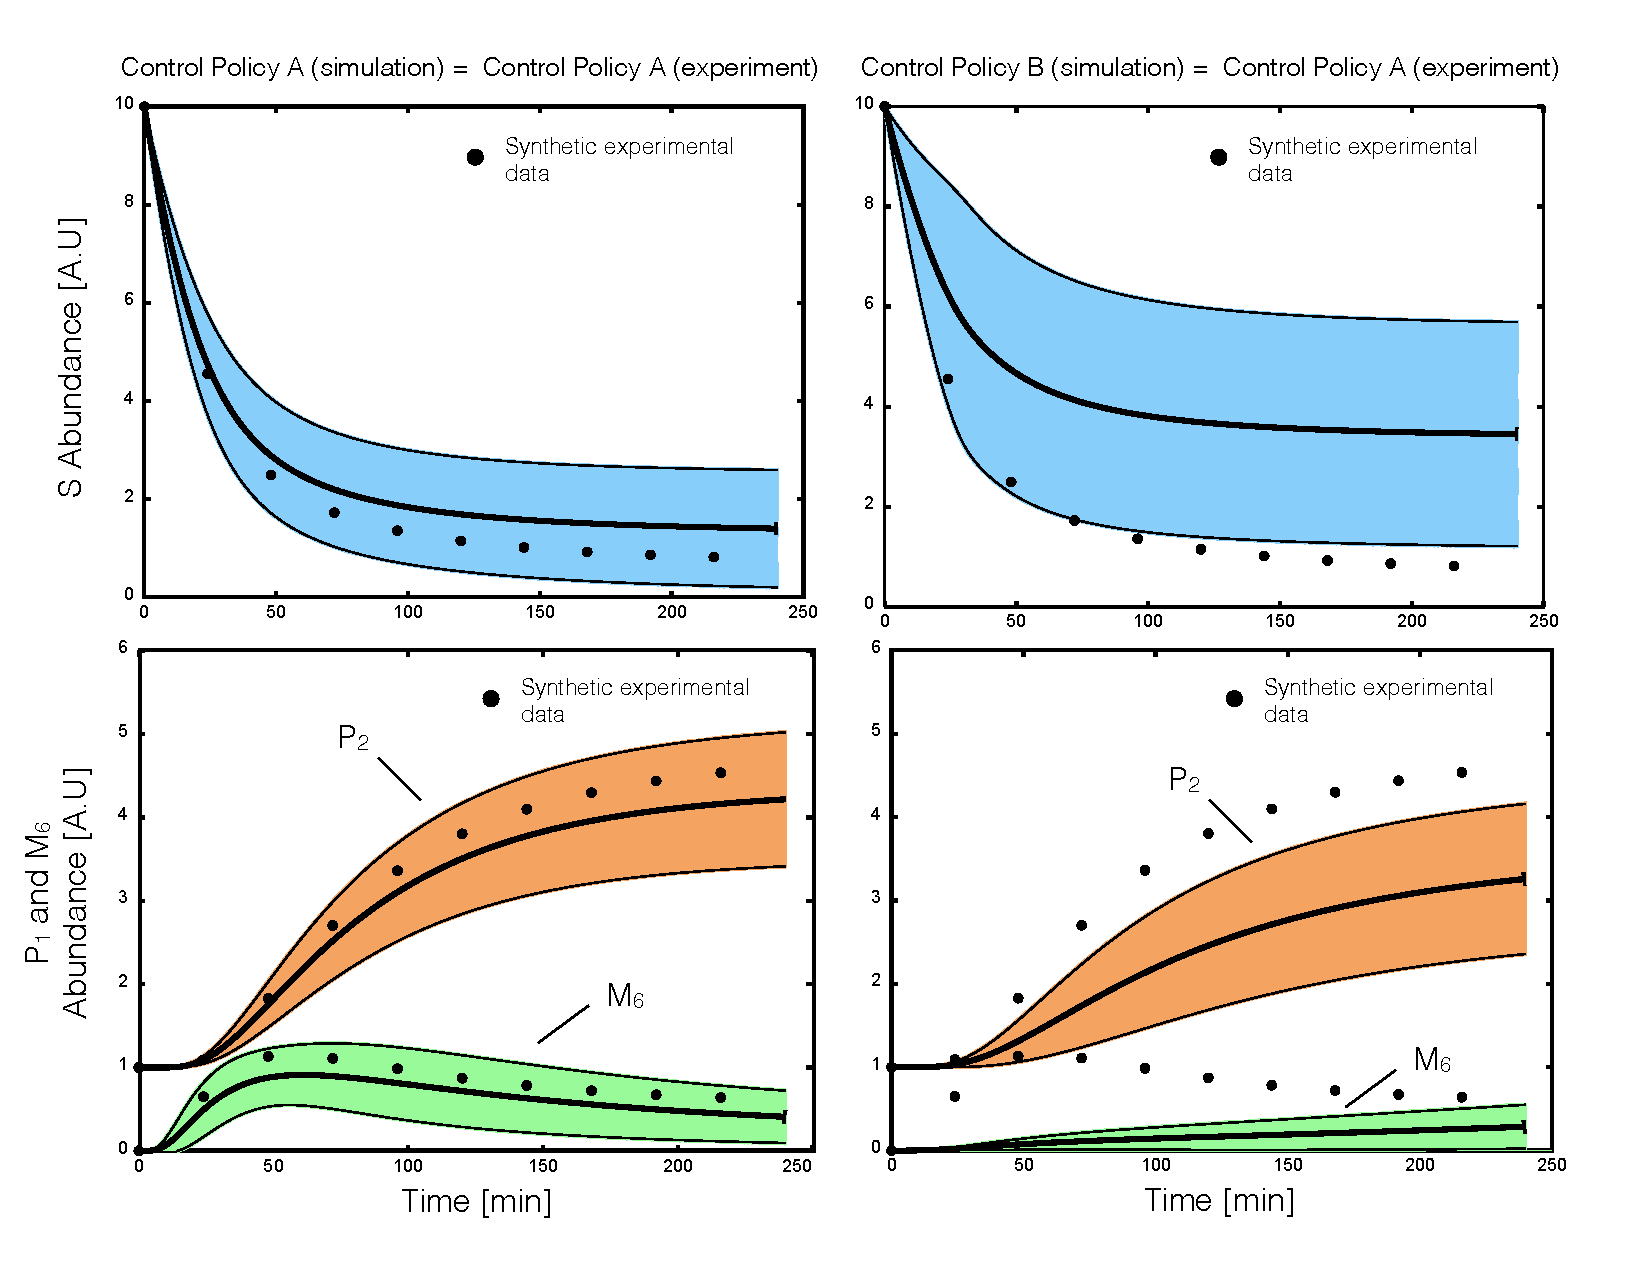
\includegraphics[width=1.0\textwidth]{./figs/Figure-5-ParameterFit.pdf}
\caption{Parameter estimation from synthetic data for the same and mismatched allosteric control logic using particle swarm optimization (PSO). 
Synthetic experimental data was generated from a hypothetical parameter set using Network A, 
where substrate $S$, end-product P$_{1}$ and intermediate M$_5$ were sampled approximately every 20 minutes. 
For cases $\textbf{A,B}$ 20 particles were initialized with randomized parameters and allowed to search for 300 iterations. 
\textbf{A,B}: PSO estimated an ensemble of parameters sets (N = 20) consistent with the synthetic experimental data assuming the correct
enzymatic and control connectivity starting from randomized initial parameters.
\textbf{C,D}: In the presence of control mismatch (Network B control policy simulated with Network A kinetic parameters) 
the ensemble of models did not describe the synthetic data. 
}\label{fig-parameter-fit}
\end{figure}

\clearpage

\begin{figure}
\centering
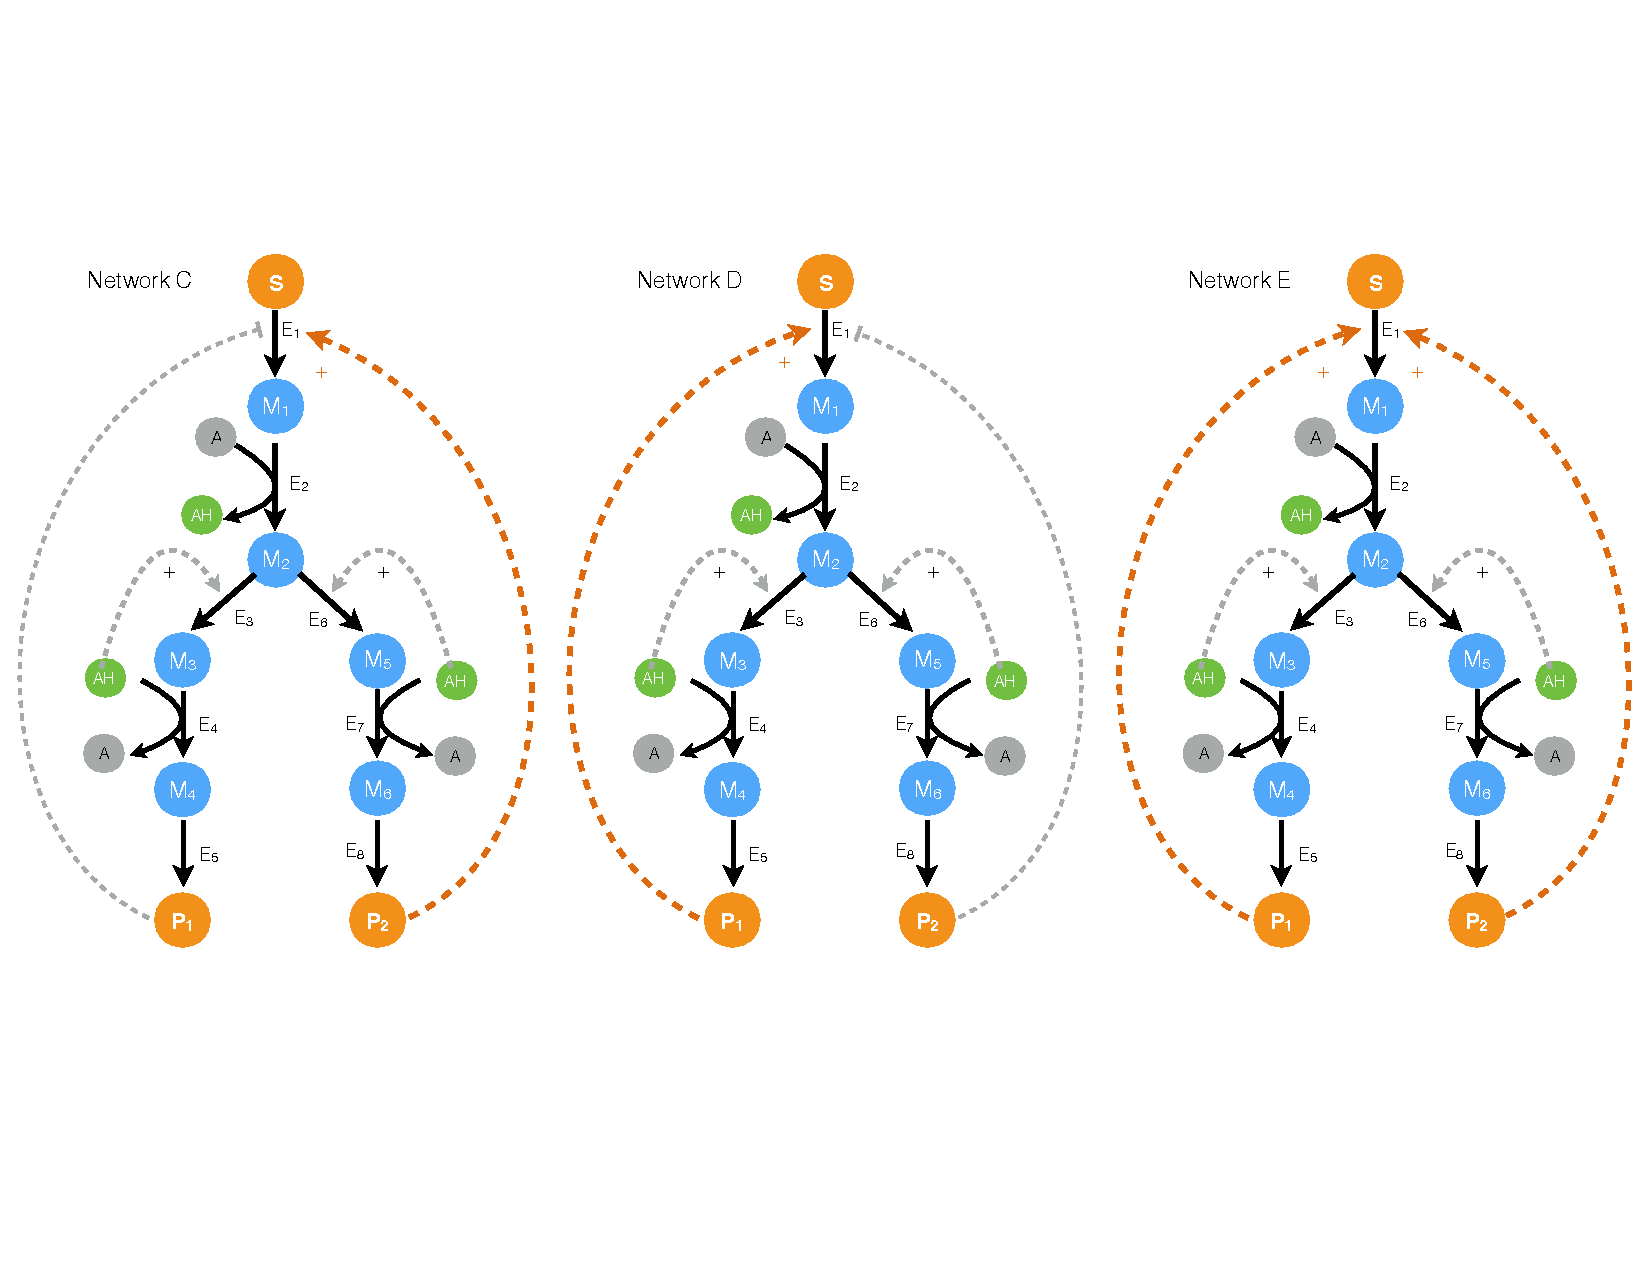
\includegraphics[width=1.0\textwidth]{./figs/Figure-6-AlternativeNetworks.pdf}
\caption{Schematic of the alternative allosteric control programs used in the structural particle swarm computation. 
Each network had the same enzymatic connectivity, initial conditions and kinetic parameters, 
but alternative feedback control structures for the first enzyme in the pathway.}\label{fig-alternative-networks}
\end{figure}

\clearpage

\begin{figure}
\centering
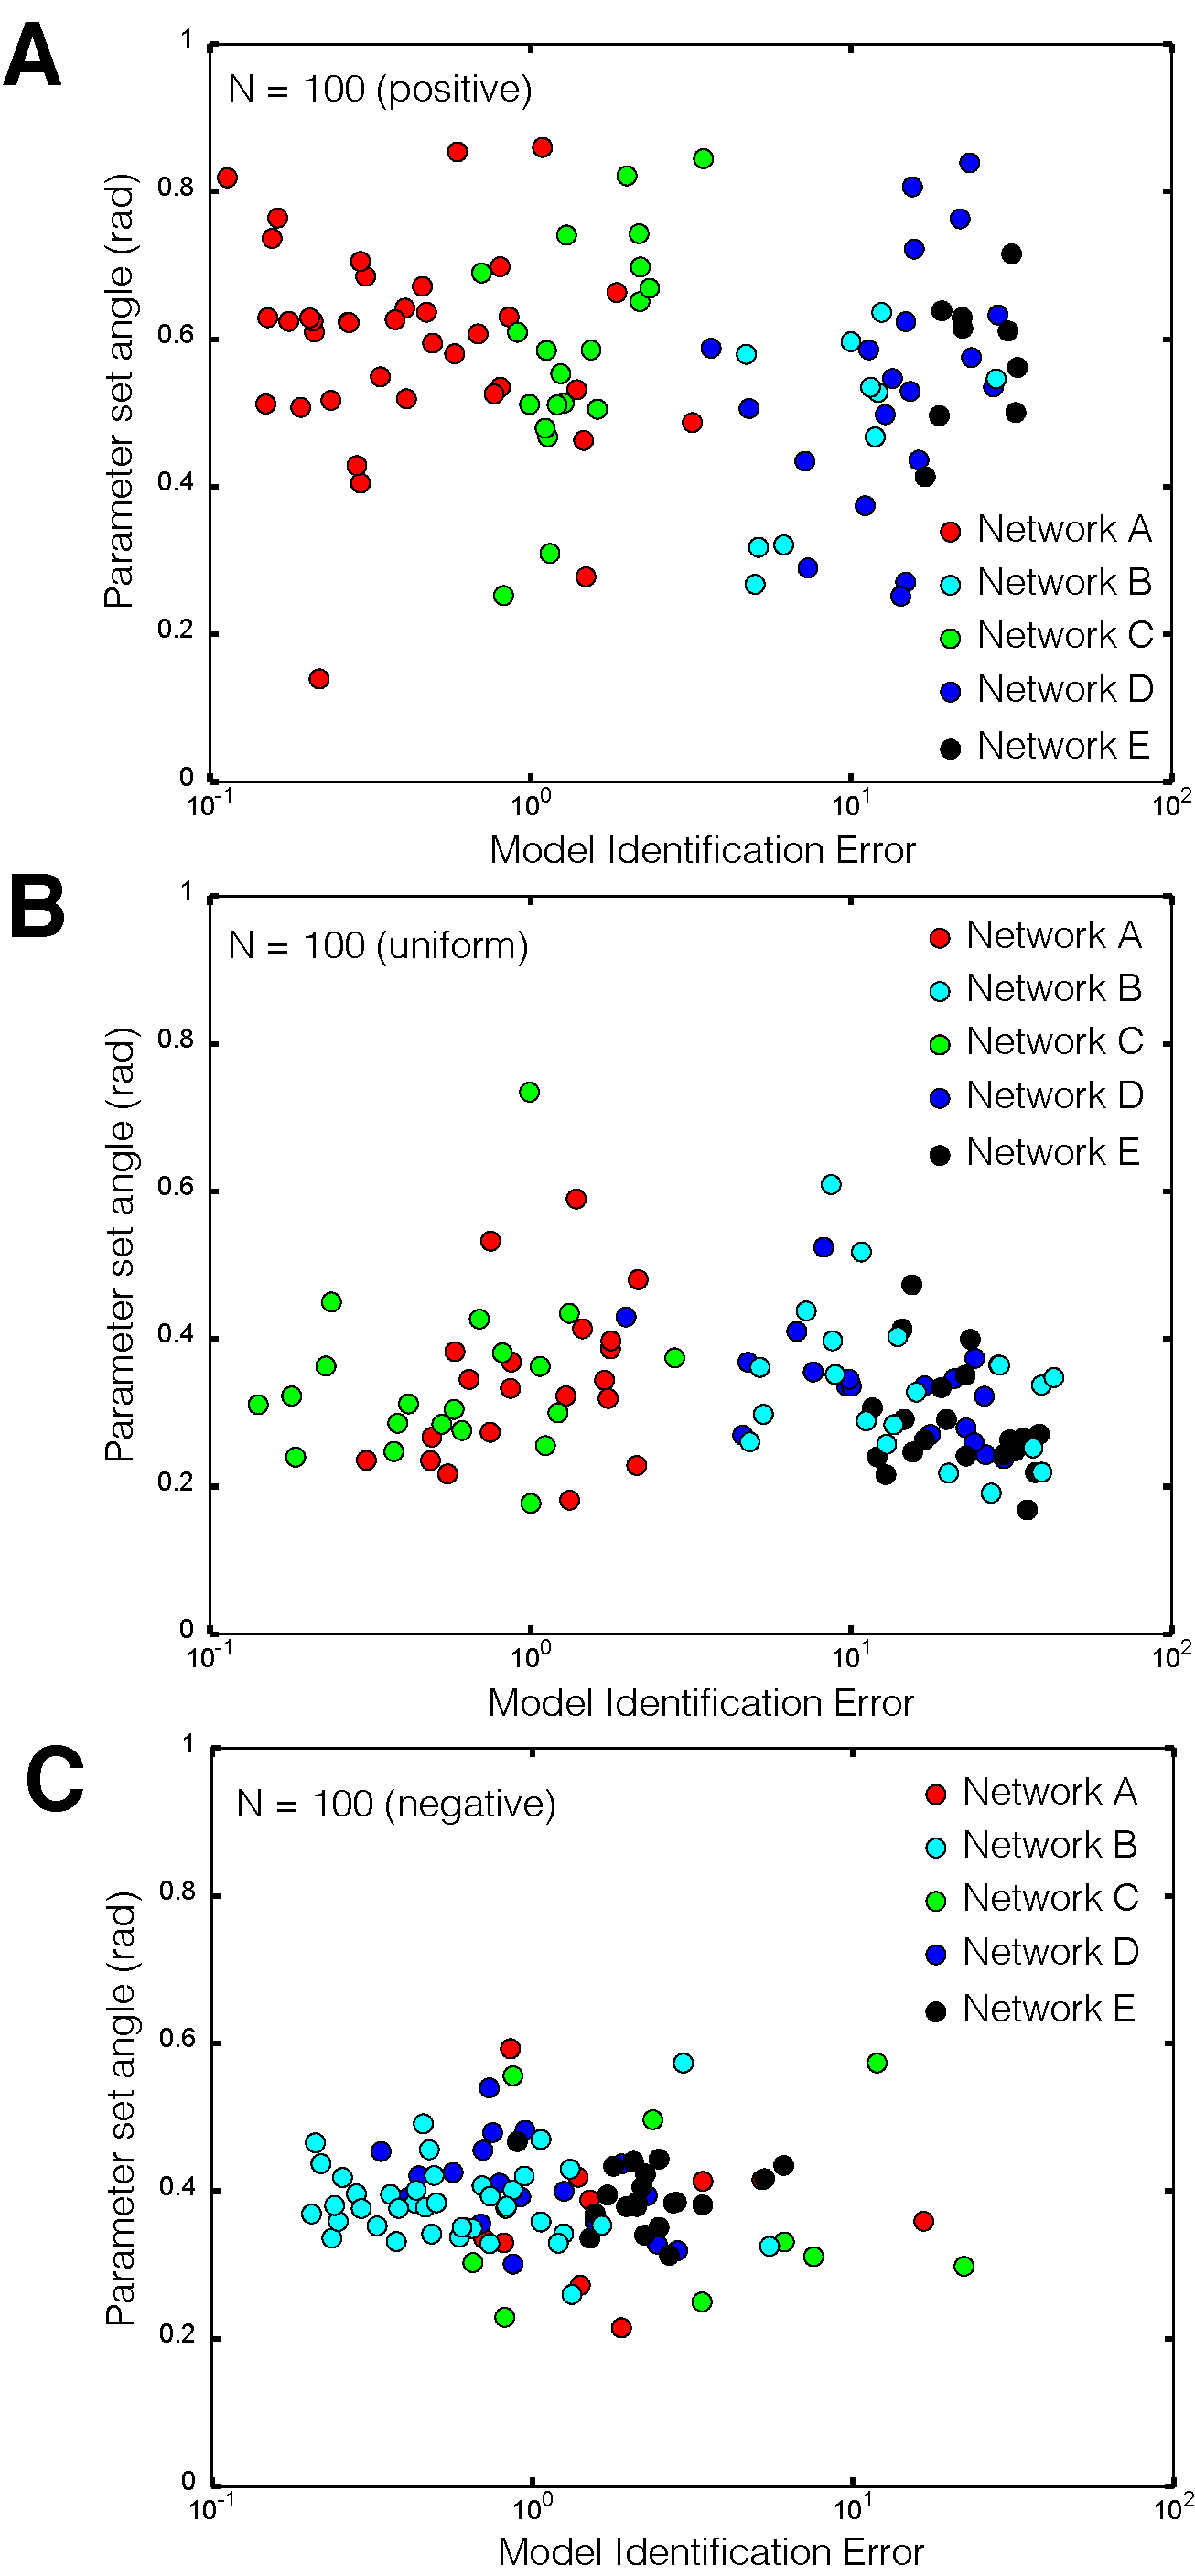
\includegraphics[width=0.5\textwidth]{./figs/Figure-7-ControlSearch.pdf}
\caption{Combined control structure and kinetic parameter search results. Think about this ...}\label{fig-control-search}
\end{figure}

\clearpage

\begin{figure}
\centering
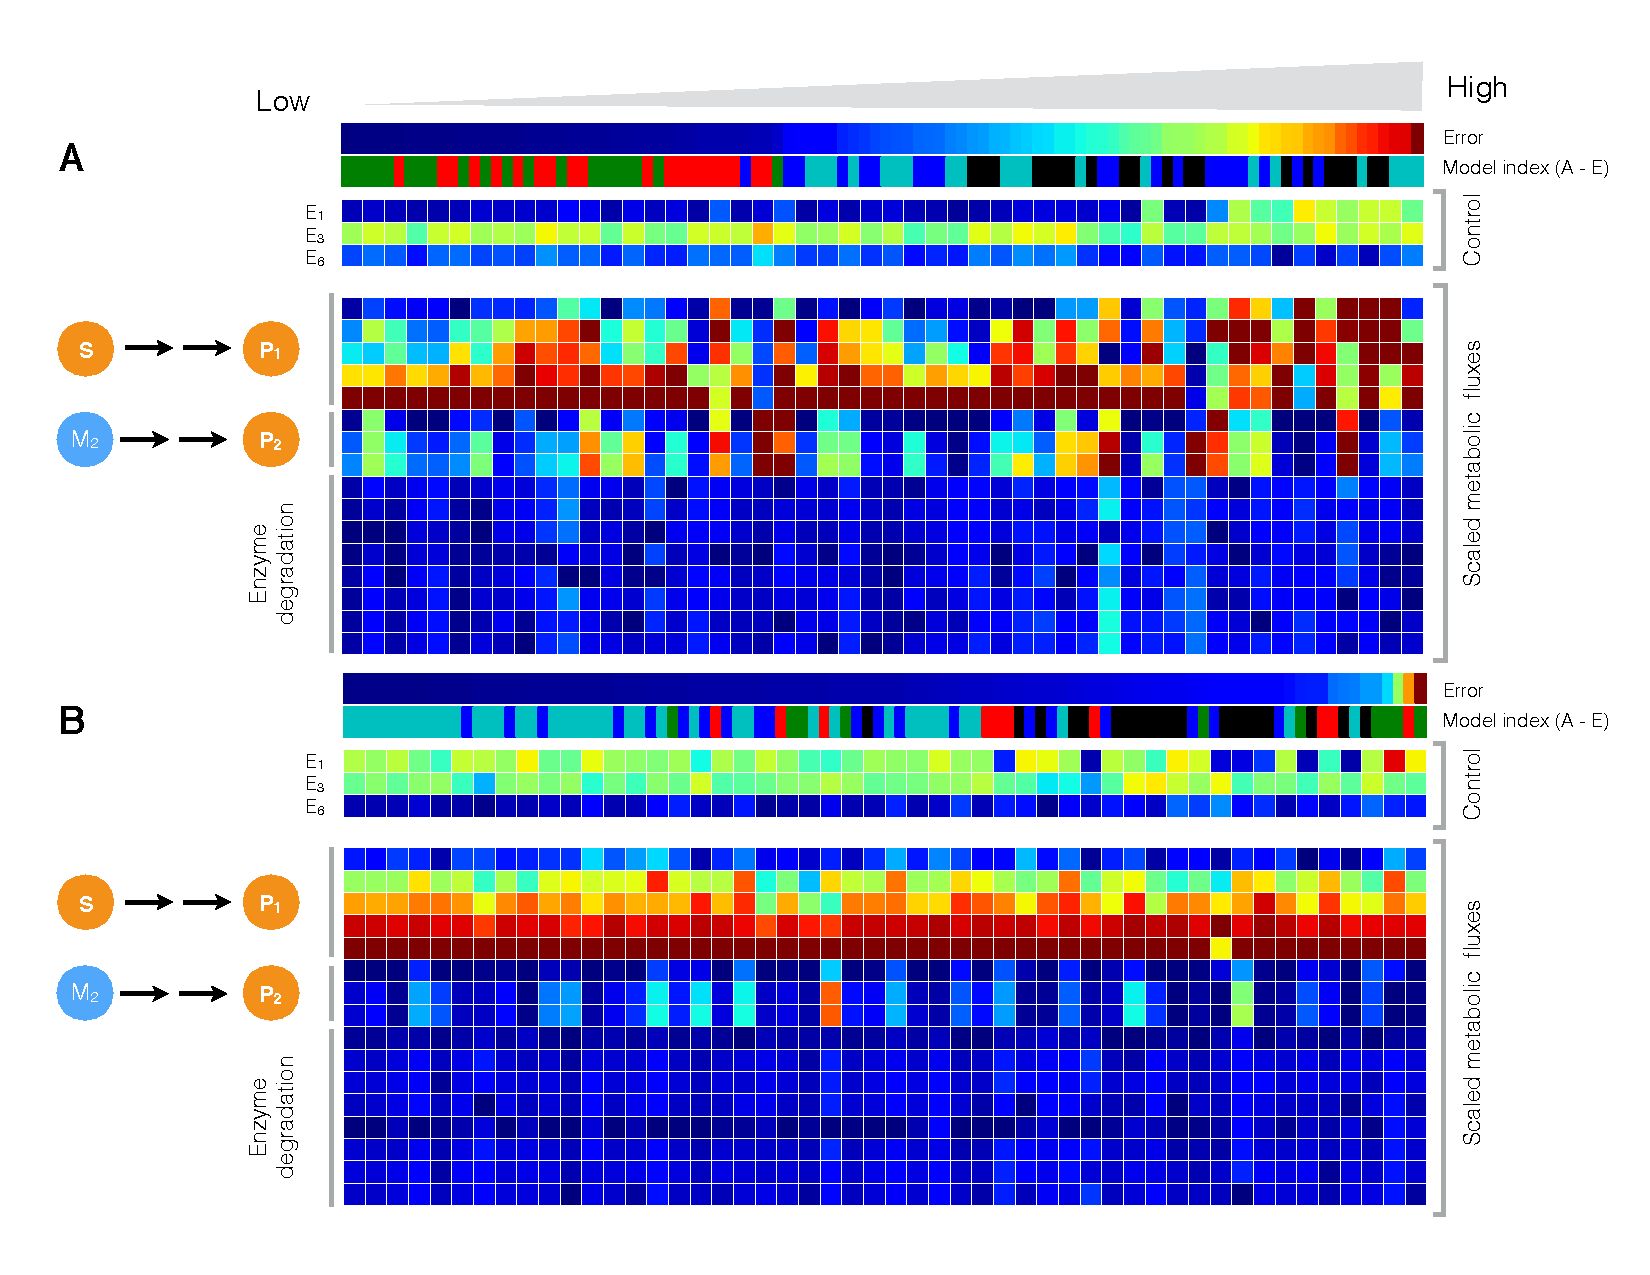
\includegraphics[width=1.0\textwidth,height=0.6\textheight]{./figs/Figure-8-Flux.pdf}
\caption{Flux and control pattern for estimated model parameters and structures. }\label{fig-flux-pattern}
\end{figure}

\clearpage

% Supplemental figures -
% Set the S- 
\renewcommand\thefigure{S\arabic{figure}}
\renewcommand\thetable{T\arabic{table}}
\renewcommand\thepage{S-\arabic{page}}
\renewcommand\theequation{S\arabic{equation}}

% Reset the counters -
\setcounter{equation}{0}
\setcounter{table}{0}
\setcounter{figure}{0}
\setcounter{page}{1}

\end{document}

